\chapter{Einleitung}

\section{Motivation}
Der Hyperloop ist ein Konzept für ein Hochgeschwindigkeitstransportsystem, das von Elon Musk \cite{tesla:Hyperloop_impact} populär gemacht wurde. Es besteht im Wesentlichen aus einer oder mehreren Kapseln, die sich durch fast luftleere Röhren bewegen. Die Idee ist, Reibung und Luftwiderstand, die zwei größten Hindernisse für hohe Geschwindigkeiten, zu minimieren.

Durch die Reduzierung von Luft- und Rollwiderstand können Hyperloop-Kapseln Geschwindigkeiten von über 600 km/h erreichen. Dies ermöglicht extrem schnelle Reisen zwischen Städten, die weit voneinander entfernt sind.

Angesichts der globalen Bemühungen zur Reduzierung der CO2-Emissionen und zur Bekämpfung des Klimawandels könnte Hyperloop eine umweltfreundlichere Alternative zu Autos und Flugzeugen bieten.

\begin{figure}[ht]
	\begin{center}
		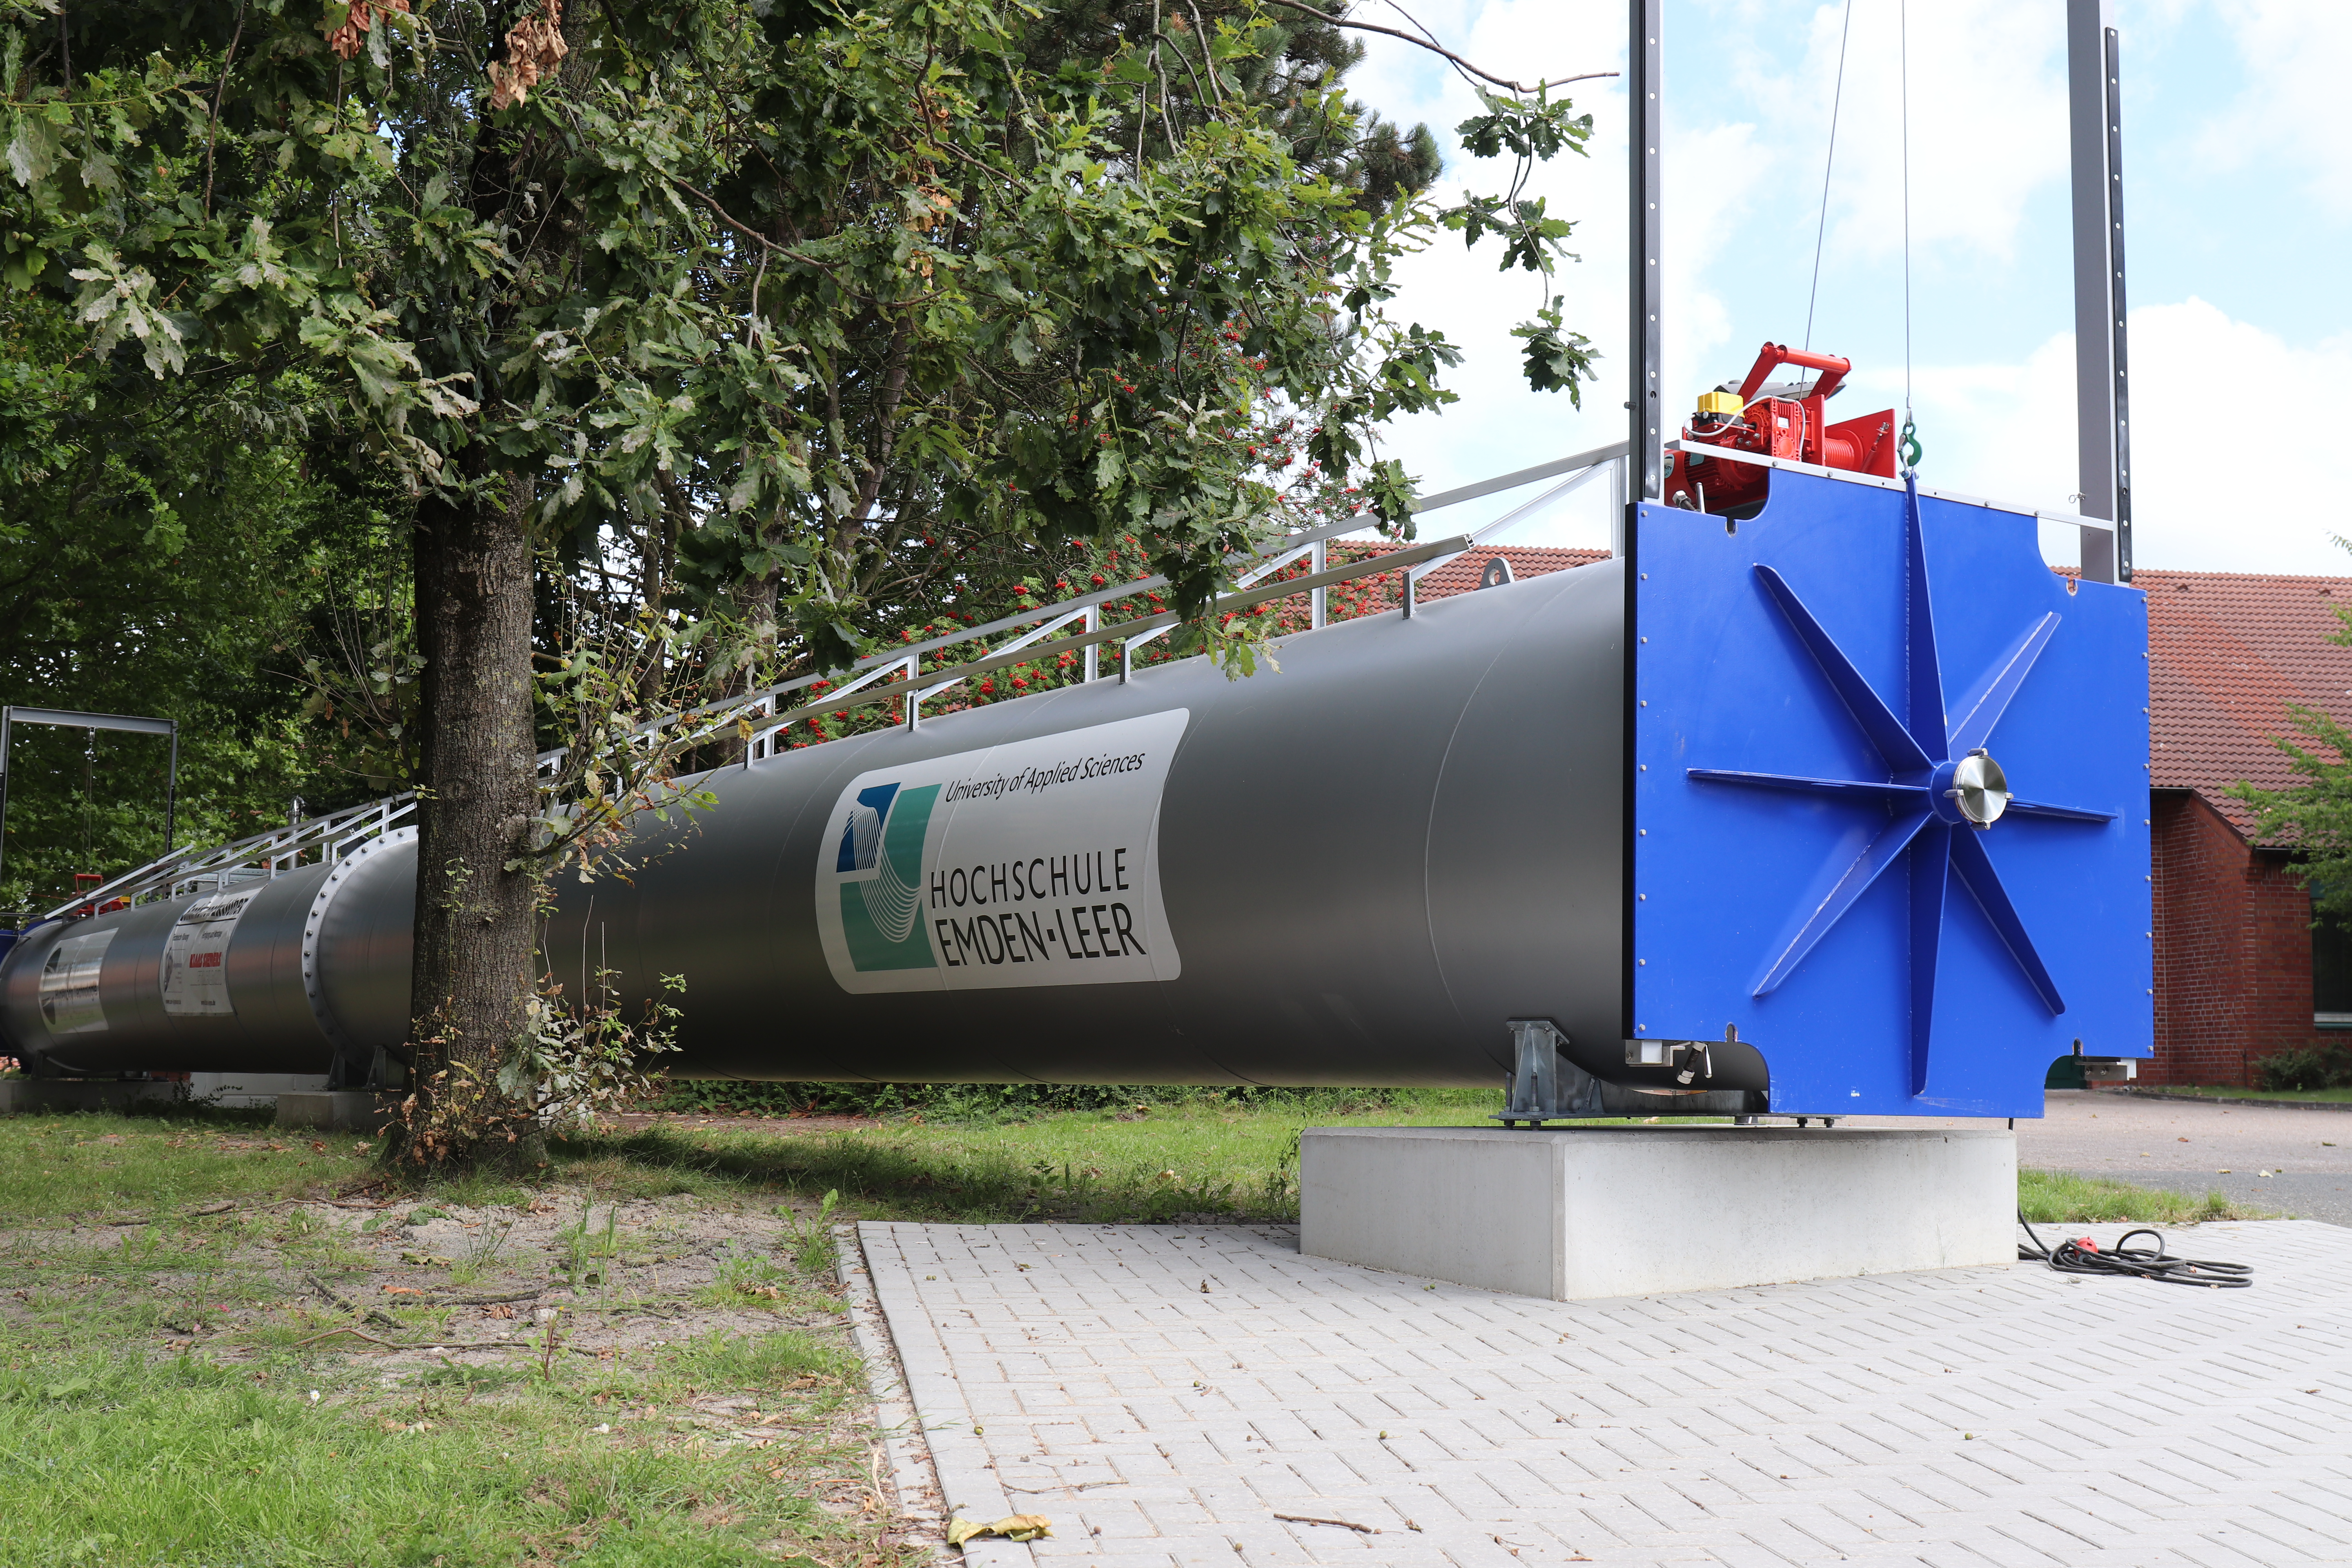
\includegraphics[width=\textwidth]{img/1_strecke/strecke_1.png}
		\caption{Hyperloop Röhre der Hochschule Emden Leer}
		\label{img_1_1:circ_bldc:1}
	\end{center}
\end{figure}
\newpage

%Das neue Design des 48-Volt-Pods ist darauf ausgelegt, Material zu transportieren. Das Konzept sieht vor, dass eine große Lagerhalle am Stadtrand die Waren annimmt und sie dann durch das unterirdische Schienennetz zu den verschiedenen Standorten befördert. Auf diese Weise soll das Verkehrsaufkommen in den Städten durch Lastkraftwagen minimiert werden.


\section{Aufgabenstellung}
Die Motivation des Projekts liegt in der Realisierung eines Fahrzeugs für den Hyperloop, welches mit einer Batterie und einem Motor betrieben werden soll. Die Steuerung soll auf dem Speedgoat erfolgen.
\newline

Im Rahmen dieses Projekts soll ein Pod für den Hyperloop mit einer Bordspannung von 48 V ausgelegt werden. Ziel ist es, die Machbarkeit dieser Spannung zu überprüfen und umzusetzen. Dazu gehören die Realisierung der Verdrahtung und der Sensorik sowie die Beschaffung der erforderlichen Bauteile. Die Logik- und Signalverarbeitung wird mithilfe von Simulink auf einem Speedgoat-System durchgeführt.


Die Steuerung erfolgt über Simulink, ein Bestandteil von Matlab. Position und Beschleunigung des Pods sollen erfasst werden, während der Motor über ein zusätzliches Steuergerät angesteuert wird.

Die Steuerung soll als eine Automatensteuerung umgesetzt werden.

Die Verdrahtung des Pods muss entsprechend der Bordspannung von 48 V realisiert werden. Dazu muss mithilfe der Software QElectroTech ein Schaltplan erstellt werden.

Es müssen alle erforderlichen Bauteile für die Umsetzung der Bordspannung, Verdrahtung und Sensorik beschafft werden.



\pagebreak

